
\documentclass{beamer}
\usepackage{HECbeamer}
\usepackage{icomma}
\usepackage{numprint}
\title[\color{white}{MATH 60604 \S~6f - Prédictions pour modèles mixtes}]{\texorpdfstring{MATH 60604 \\Modélisation statistique \\ \S~6f - Prédictions pour modèles mixtes}{MATH 60604 \\Modélisation statistique \\ \S~6f - Prédictions pour modèles mixtes}}
\author{Léo Belzile}
\institute{HEC Montréal\\
Département de sciences de la décision}
\date{}

\begin{document}
\frame{\titlepage}
\section{Prédiction pour modèles à effets aléatoires}
\begin{frame}
\frametitle{Prédiction}
\bi
\item Les effets
aléatoires $\bs{b}$ sont des \alert{variables aléatoires} et non pas des paramètres (c'est-à dire
des quantités fixes, mais inconnues).
\item On peut toutefois obtenir des \alert{prédictions} pour
ces effets aléatoires.
% \item Attention, ne pas confondre \alert{prédiction} avec \alert{estimation} car il s'agit de variables aléatoires.
\item Une fois qu'on a prédit les effets aléatoires $\bs{b}$ et estimé les paramètres des effets fixes $\bs{\beta}$, on peut prédire la moyenne conditionnelle des $\bs{Y}$.
\ei
\end{frame}


\begin{frame}

\frametitle{Prédiction: modèle \textbf{sans} effet aléatoire}
\bi
\item \alert{S'il n'y a pas d'effets aléatoires dans le modèle} (par exemple si on a
seulement utilisé une structure de covariance pour les erreurs), alors on est
dans la même situation qu'en régression linéaire ordinaire.
\item C'est-à-dire, la
prédiction pour $Y_{ij}$ est
\begin{align*}
\hat{Y}_{ij}=\hat{\beta}_0 + \hat{\beta}_1\mathrm{X}_{ij1} + \ldots + \hat{\beta}_p\mathrm{X}_{ijp}.
\end{align*}
\item Cette quantité est aussi l'estimation des \alert{moyennes} (au niveau
de la \alert{population}) de la variable réponse.
\ei
\end{frame}


\begin{frame}
\frametitle{Prédiction: modèle \textbf{avec} effets aléatoires}
\bi
\item S'il y a des effets aléatoires dans le modèle, l'estimation
de la \alert{moyenne marginale} (au niveau de la \alert{population}) de la variable réponse pour un individu ayant les caractéristiques de l'individu $j$ du
groupe $i$ est
\begin{align*}
\hat{Y}_{ij}=\hat{\beta}_0 + \hat{\beta}_1\mathrm{X}_{ij1} + \ldots + \hat{\beta}_p\mathrm{X}_{ijp}.
\end{align*}


\item On peut aussi prédire des
\alert{valeurs} de la variable réponse de l'individu $j$ du groupe $i$: par exemple, dans un modèle avec effet aléatoire sur l'ordonnée à l'origine $b_i$ du groupe $i$,
 \begin{align*}
\hat{Y}_{ij}=\hat{\beta}_0 +\hat{b}_{i} + \hat{\beta}_1\mathrm{X}_{ij1} + \ldots + \hat{\beta}_p\mathrm{X}_{ijp}.
\end{align*}
\ei 
\end{frame}
\begin{frame}
\frametitle{Prédiction: modèle \textbf{avec} effets aléatoires}
\bi
\item Par contre, si on désire obtenir une prédiction pour une observation d'un \alert{nouvel}
individu/groupe dont les caractéristiques ne sont pas présentes dans l'échantillon d'apprentissage, alors on n'a
pas le choix que d'utiliser la prédiction de la moyenne, car l'estimation de l'effet aléatoire n'est pas disponible pour ce nouveau groupe.
\ei
\end{frame}

\begin{frame}[fragile]
\frametitle{Prédiction des effets aléatoires}

\begin{tcolorbox}[colback=white, colframe=hecblue, title=Code \SASlang pour l'ordonnée à l'origine aléatoire]
\begin{footnotesize}
\begin{verbatim}
proc mixed data=modstat.mobilisation;
class idunite;
model mobilisation = sexe anciennete agegest nunite / solution;
random intercept / subject=idunite type=vc solution;
ods output Mixed.SolutionR=re;
run;
\end{verbatim}
\end{footnotesize}
\end{tcolorbox}
\begin{small}L'option \code{solution} à la commande \code{random} est utilisée pour avoir les
prédictions des effets aléatoires dans la sortie. La commande \code{ods output}
sauvegarde ces derniers afin qu'on puisse produire des diagnostics graphiques pour les effets aléatoires.
\end{small}
\end{frame}

\begin{frame}
\frametitle{Prédiction des effets aléatoires}
\begin{center}
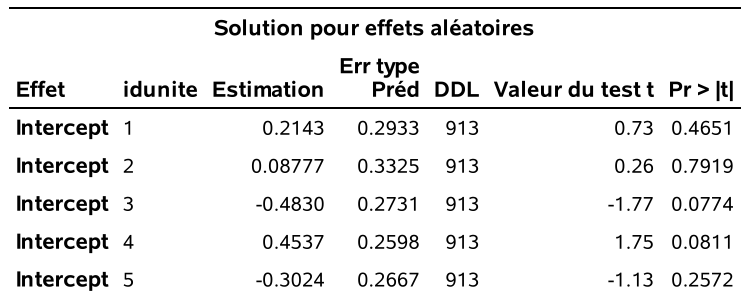
\includegraphics[width = 0.7\linewidth]{img/c6/diapos7-e19}
\begin{align*}
 \vdots
\end{align*}
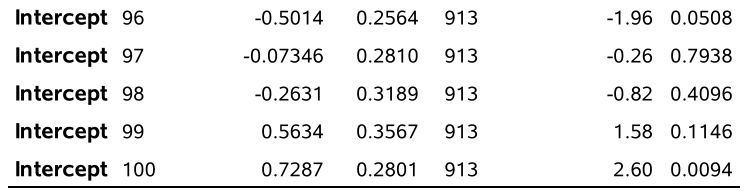
\includegraphics[width = 0.7\linewidth]{img/c6/diapos7-e20}
\end{center}
\end{frame}

% \begin{frame}
% \frametitle{Predictions for the random effect terms of the first three units}
%
% \begin{center}
% \includegraphics[scale=0.5]{img/c6/long118.pdf}
% \end{center}
% \begin{small} Only part of the table is shown here: the full table includes predictions for all $100$ units in the dataset. \end{small}
% \end{frame}
%
\begin{frame}
\frametitle{Vérification des effets aléatoires}
on peut tracer un histogramme et produire un diagramme quantile-quantile normal des ordonnées à l'origine prédites.
\begin{center}
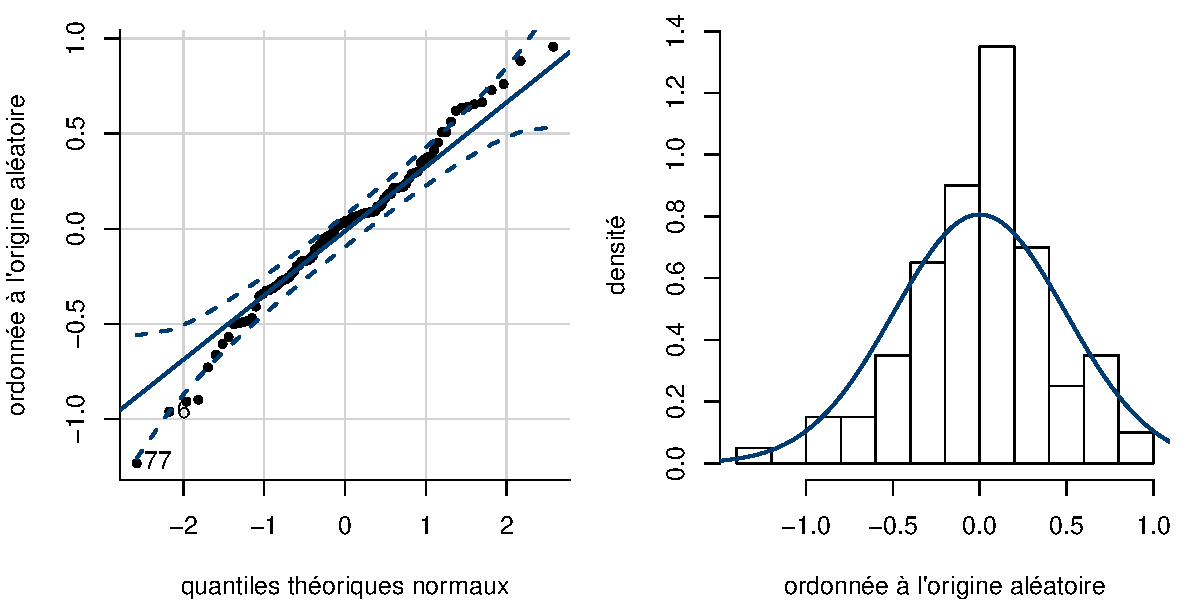
\includegraphics[width = 0.8 \linewidth]{img/c6/07-mixed-diagran_fr}
\end{center}
Ces diagnostics graphiques permettent de vérifier l'hypothèse de normalité des effets aléatoires (considérez-les comme des diagnostics des résidus supplémentaires). Il est important de noter que, par construction, la moyenne des effets aléatoires est toujours zéro.
\end{frame}

% \begin{frame}
% \frametitle{Scatterplot of the random intercept $b_i$ as a function of $b_{1i}$}
%
% \begin{center}
% \includegraphics[scale=0.35]{img/c6/long121.pdf}
% \end{center}
% \bi
% \item We assumed that the two effects are independent.
% \item This assumption can be relaxed in \code{proc mixed} by setting, e.g., \code{type = un}.
% \ei
% \end{frame}

\begin{frame}[fragile]
\frametitle{Prédiction de nouvelles variables cibles}
\bi
\item Avec \code{\code{proc mixed}}, on peut sauvegarder les valeurs \alert{pour toutes les observations dans un jeu de données}:
\bi
\item prédiction de la moyenne de la population (effets fixes),
\item prédictions individuelles (effets fixes et aléatoires).
\ei
\item Ceci se fait en ajoutant les options \code{outpm}
et \code{outp}, respectivement, à la commande \code{model}.
\item \textbf{Truc \SASlang{}}: Si vous désirez obtenir des prédictions pour des nouveaux
individus, il suffit de les inclure 
dans la base de données en laissant des
valeurs manquantes (``.'' pour \SASlang{}) pour la variable réponse. Ainsi, ces individus
ne vont pas être utilisés pour ajuster le modèle, mais des valeurs prédites pour
eux seront quand même produites.
\ei
\end{frame}

\begin{frame}[fragile]
\frametitle{Prédiction pour de nouveaux employés}
On veut obtenir des prédictions pour deux nouveaux employés, l'un qui fait partie d'une unité connue (\code{idunite=1}) et un autre qui fait partie d'une unité absente des données originales (\code{idunite=101}).
\begin{tcolorbox}[colback=white, colframe=hecblue, title=Code \SASlang pour imputer deux nouvelles observations]
\begin{small}
\begin{verbatim}
data newdata;
input nunite idunite idemployee anciennete sexe
     mobilisation agegest;
cards;
9 1 10 5 0 . 40
9 101 1 5 0 . 40;
run;

/* Fusionner observations */
data mobilisation;
set modstat.mobilisation newdata;
run;
\end{verbatim}
\end{small}
\end{tcolorbox}
\end{frame}

\begin{frame}[fragile]
\frametitle{Ajustement du modèle et obtention des prédictions}
\begin{tcolorbox}[colback=white, colframe=hecblue, title=Code \SASlang pour obtenir des prédictions du modèle mixte]
\begin{verbatim}
proc mixed data=mobilisation;
class idunite;
model mobilisation = sexe anciennete agegest nunite
     / solution outp=prediction outpm=mean;
random intercept / subject=idunite type=vc;
run;
\end{verbatim}
\end{tcolorbox}
\bi
\item  Le jeu de données \code{mobilisation} contient les $1018$ observations, mais seulement les $1016$ observations originales seront utilisées pour ajuster le modèle.
\item Par contre, les prédictions seront produites pour toutes les $1018$ observations dans les fichier \texttt{mean} et \texttt{prediction}.
\ei
\end{frame}

\begin{frame}[fragile]
\frametitle{Moyenne de la population pour les deux nouveaux individus}
Sortie du fichier \texttt{mean}:
\begin{center}
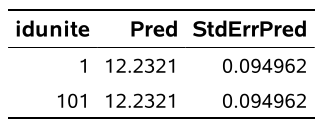
\includegraphics[width = 0.4\linewidth]{img/c6/diapos7-e21}
\end{center}
\bi
\item La moyenne de la population ($12,23$) est la même pour les deux individus parce que seuls les effets fixes sont pris en compte et les employés ont les même valeurs explicatives.
\ei
\end{frame}

\begin{frame}[fragile]
\frametitle{Prédictions pour deux nouveaux individus}

Sortie du fichier \texttt{prediction}:
\begin{center}
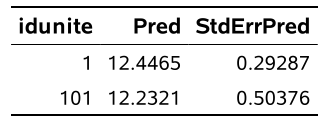
\includegraphics[width = 0.4\linewidth]{img/c6/diapos7-e22}
\end{center}
\bi
\item Cette fois ci, les effets aléatoires sont utilisés pour autant qu'ils soient disponibles. Puisque l'unité $1$ était présente lors de l'ajustement, l'effet aléatoire du groupe est utilisé dans la prédiction ($12,45$).
\item En revanche, l'unité
$101$ n'était pas disponible et donc la prédiction pour l'employé de l'unité $101$ est basée seulement sur la moyenne marginale de la population (effets fixes) ($12.23$).
\item Dans les deux cas, les erreurs-type des prédictions individuelles sont plus larges que celles de la moyenne, ce qui réflète l'incertitude additionnelle des erreurs et des effets aléatoires.
\ei
\end{frame}
\end{document}
